% @Author: AnthonyKenny98
% @Date:   2020-02-28 15:02:19
% @Last Modified by:   AnthonyKenny98
% @Last Modified time: 2020-03-01 15:49:31

\todo[inline]{Brief introduction outlining purpose of performance analysis}

\subsection{Methodology}
    To restate, the aim of this thesis is to design a computer processor with reduced execution time of motion planning algorithms, such as \ac{RRT}. As such, it is important to understand the elements of the algorithm that have the highest percentage of CPU execution time. To determine this, it was necessary to implement my own, naive but typical, \ac{RRT} in C. This program could then be compiled and analysed using a software performance profiling tool. With this, I could design experiments to determine the critical RRT functions (those occupying a majority of CPU time) and see how this varies given different parameters.
    \todo[inline]{Outline of method of analysis. Something better than the above}

    \subsubsection*{VTune Profiler}
    \label{subsubsection:vtune}
        VTune Profiler performance profiler is an application for software performance analysis. It provides functionality to examine hot-spots for CPU execution time through a top down analysis, shown below in Figure \ref{figure:VTuneTopDown}. As can be seen from the figure, the top down analysis tool shows the percentage of CPU time taken up by each function. I used this tool to profile the algorithm's performance as I changed certain parameters.
        \todo[inline]{Rewrite the above}
        % @Author: AnthonyKenny98
% @Date:   2020-02-23 14:33:19
% @Last Modified by:   AnthonyKenny98
% @Last Modified time: 2020-02-23 14:36:06

\begin{figure}[H]
\begin{center}
    \missingfigure[figwidth=\linewidth]{Screenshot of VTune Top Down Analysis (Maybe)}
    \caption{VTune Amplifier TopDown Analysis Example}
    \label{figure:VTuneTopDown}
\end{center}
\end{figure}

    \subsubsection*{Internal Timing}
        The limitation of VTune Profiler is that it can only profile software running on Intel processors, which implement the x86-64 \ac{ISA}. As such, when the time comes to analyse performance of the software running on a RISC-V processor, another method will be required. A simple and effective way of measuring execution performance is to insert timing functionality into the software itself. \\

        \todo[inline]{Provide or link to appendix of explanation of internal timing}

    \subsubsection*{Comparison}
        Before proceeding to use either of these methods to profile the software implementation of \ac{RRT}, it was important to verify that the two methods yielded similar results for the same program. Table \ref{table:timing_calibration} summarizes the results of analysis of a simple C executable. The program calls 5 functions, $\{A, B, C, D, E\}$, each a simple iteration in which a integer is incremented. Since the Internal Timing method returned similar results to the (trusted) VTune Profiler, it was considered to be a reliable method. While it was encouraging to see both methods returned similar results for absolute execution time, the more important metric was the similarity in percentage of total execution time.

        \begin{table}[H]
\begin{center}
\begin{tabular}{|m{0.1\linewidth}|m{0.18\linewidth}|m{0.18\linewidth}|m{0.18\linewidth}|m{0.18\linewidth}|}
\hline
\multirow{2}{*}{function} & \multicolumn{2}{c|}{Vtune Profiler} & \multicolumn{2}{c|}{Internal Timing} \\
\cline{2-5}
            & time (s)  & time (\% total) & time (s) & time (\% total)    \\
\hline
A       & 0.488     & 57.4\%        & 0.497 & 57.6\%           \\
B       & 0.2       & 23.5\%        & 0.198 & 23.1\%           \\
C       & 0.102     & 12.0\%        & 0.099 & 11.5\%           \\
D       & 0.048     & 5.7\%         & 0.049 & 5.6\%            \\
E       & 0.012     & 1.4\%         & 0.019 & 2.2\%            \\
\hline
\end{tabular}
\end{center}
\caption{Comparison of Timing Methods}
\label{table:timing_calibration}
\end{table}

    \subsubsection*{Experimental Design}
        In profiling \ac{RRT} in software, the goal was to find the critical task across different values of $K$ and sizes of configuration space. Multiple tests were run, varying these two constraints, to find this critical function. The results of this analysis can be found in Section \ref{section:rrt_analysis_results}.

\subsection{Results}
\label{section:rrt_analysis_results}
    Figure \ref{fig:rrt_profiling} shows the profile of functions within \ac{RRT}, for $100 \leq K \leq 10000$, and cubic configuration spaces with dimensions $\{4, 8, 16, 32\}$. Each subfigure shows a similar profile, with the \% of CPU Execution Time taken by findNearestNode increasing with $K$. This is to be expected. \todo{Explanation of time complexity}However, it is also seen that edgeCollisions increases with larger configuration spaces, taking up the overwhelming majority of execution time for a 32x32x32 configuration space.
    
    \newpage
    % @Author: AnthonyKenny98
% @Date:   2020-02-29 14:51:44
% @Last Modified by:   AnthonyKenny98
% @Last Modified time: 2020-03-01 08:07:28
\begin{figure}[H]
\begin{center}

    % Subfigure A
    \begin{subfigure}{\textwidth}
    \begin{center}
    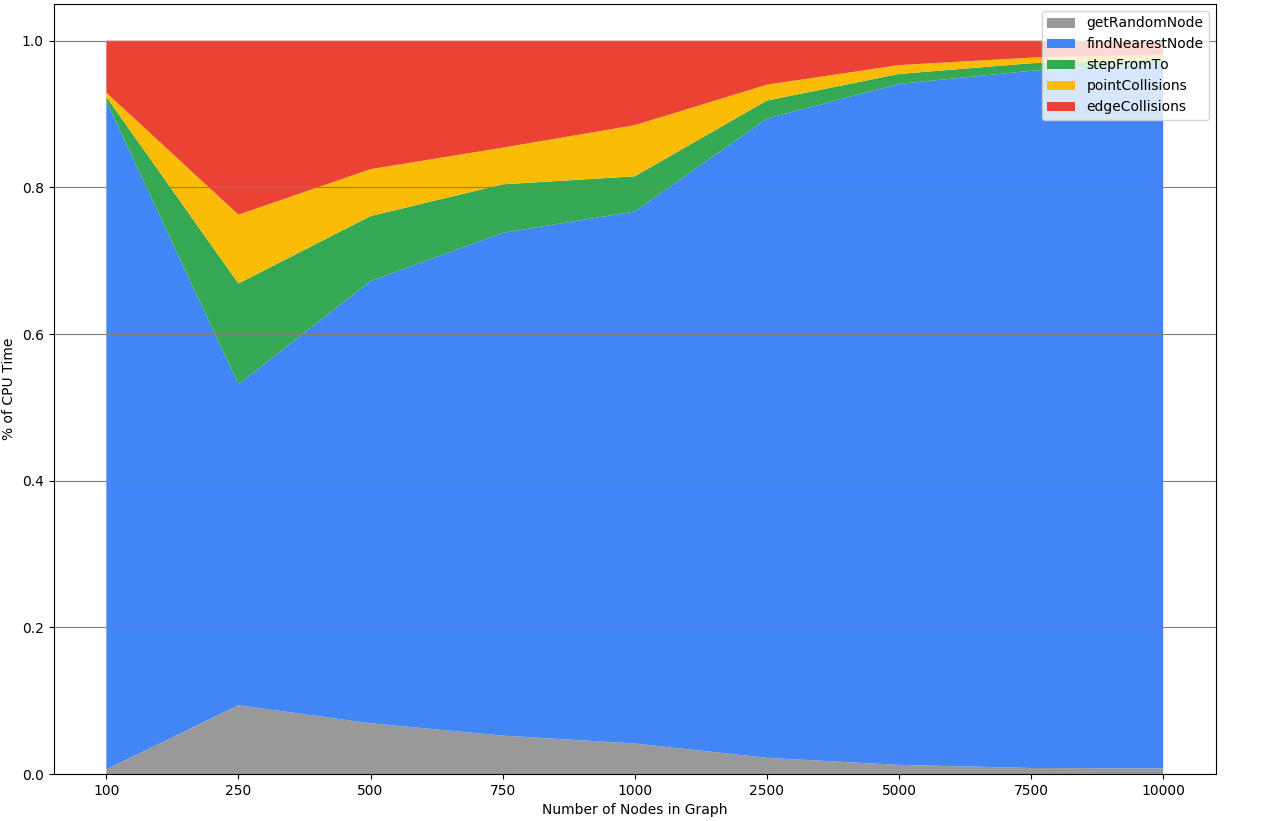
\includegraphics[width=\linewidth,height=0.3\paperheight]{chapters/chapter2/img/profiling/4x4x4/performance.png}
    \caption{4x4x4 Configuration Space}
    \label{subfig:4x4x4rrt}
    \end{center}
    \end{subfigure}
    % 
    % Subfigure B
    \begin{subfigure}{\textwidth}
    \begin{center}
    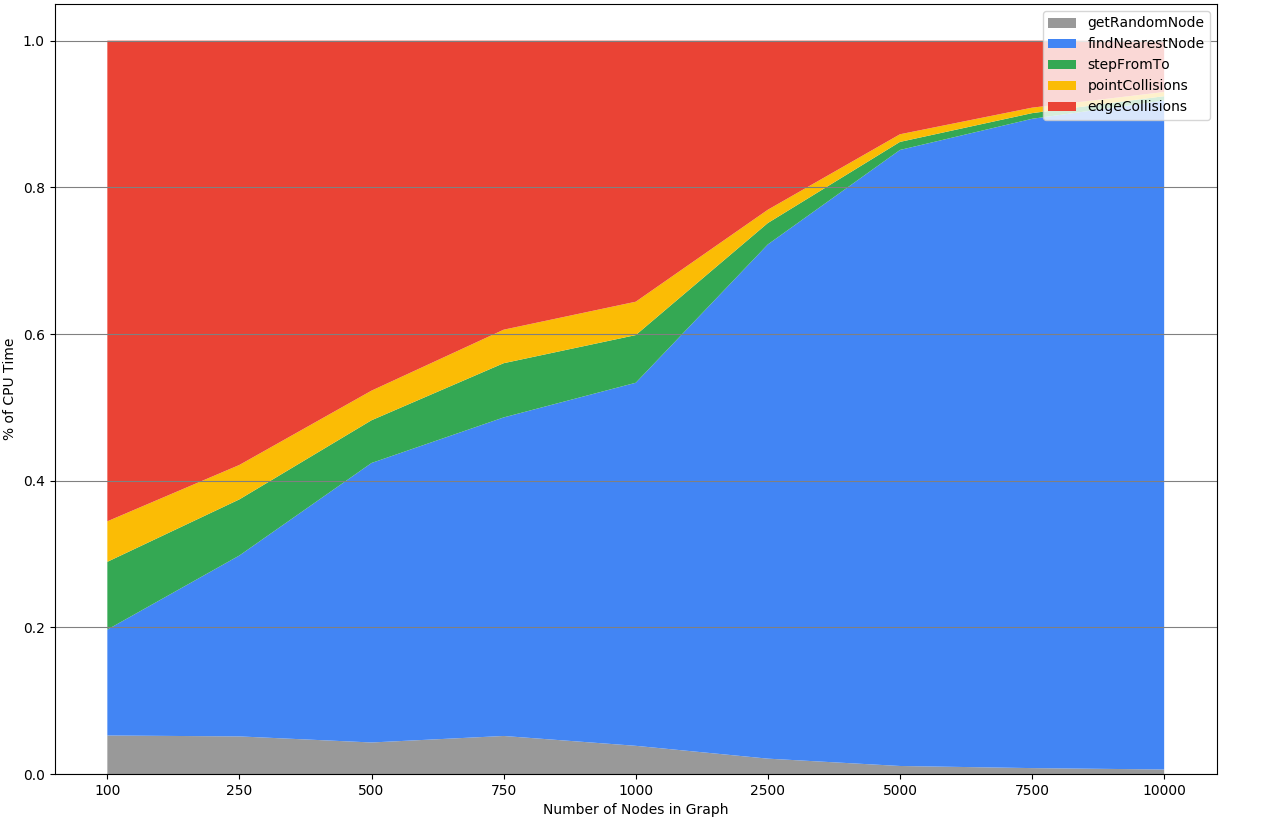
\includegraphics[width=\linewidth,height=0.3\paperheight]{chapters/chapter2/img/profiling/8x8x8/performance.png}
    \caption{8x8x8 Configuration Space}
    \label{subfig:8x8x8rrt}
    \end{center}
    \end{subfigure}
    % Caption and Label
    \caption{\ac{RRT} Functions as a \% of Total CPU Exectution Time}
\end{center}
\end{figure}

\newpage
\begin{figure}[H]\ContinuedFloat
\begin{center}
    % 
    % Subfigure C
    \begin{subfigure}{\textwidth}
    \begin{center}
    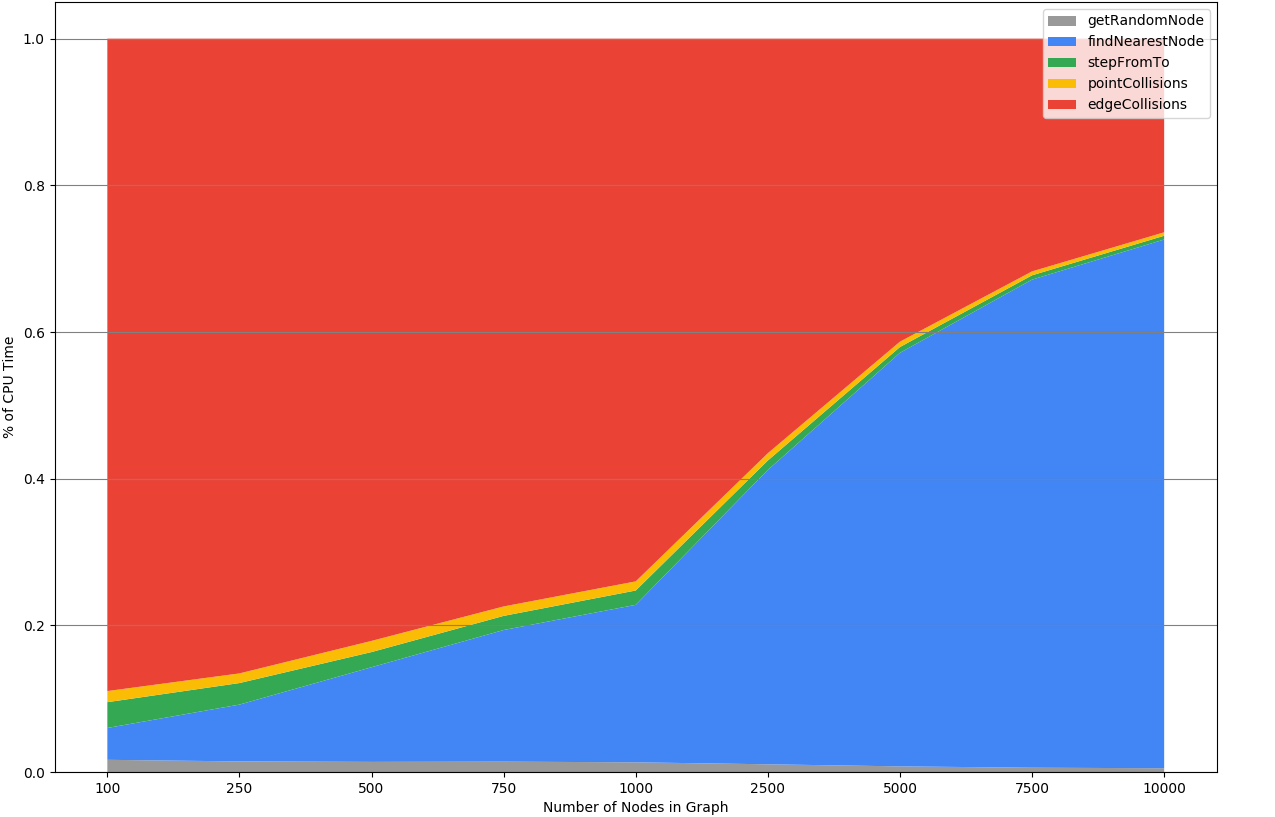
\includegraphics[width=\linewidth,height=0.3\paperheight]{chapters/chapter2/img/profiling/16x16x16/performance.png}
    \caption{16x16x16 Configuration Space}
    \label{subfig:16x16x16rrt}
    \end{center}
    \end{subfigure}
    % 
    % Subfigure D
    \begin{subfigure}{\textwidth}
    \begin{center}
    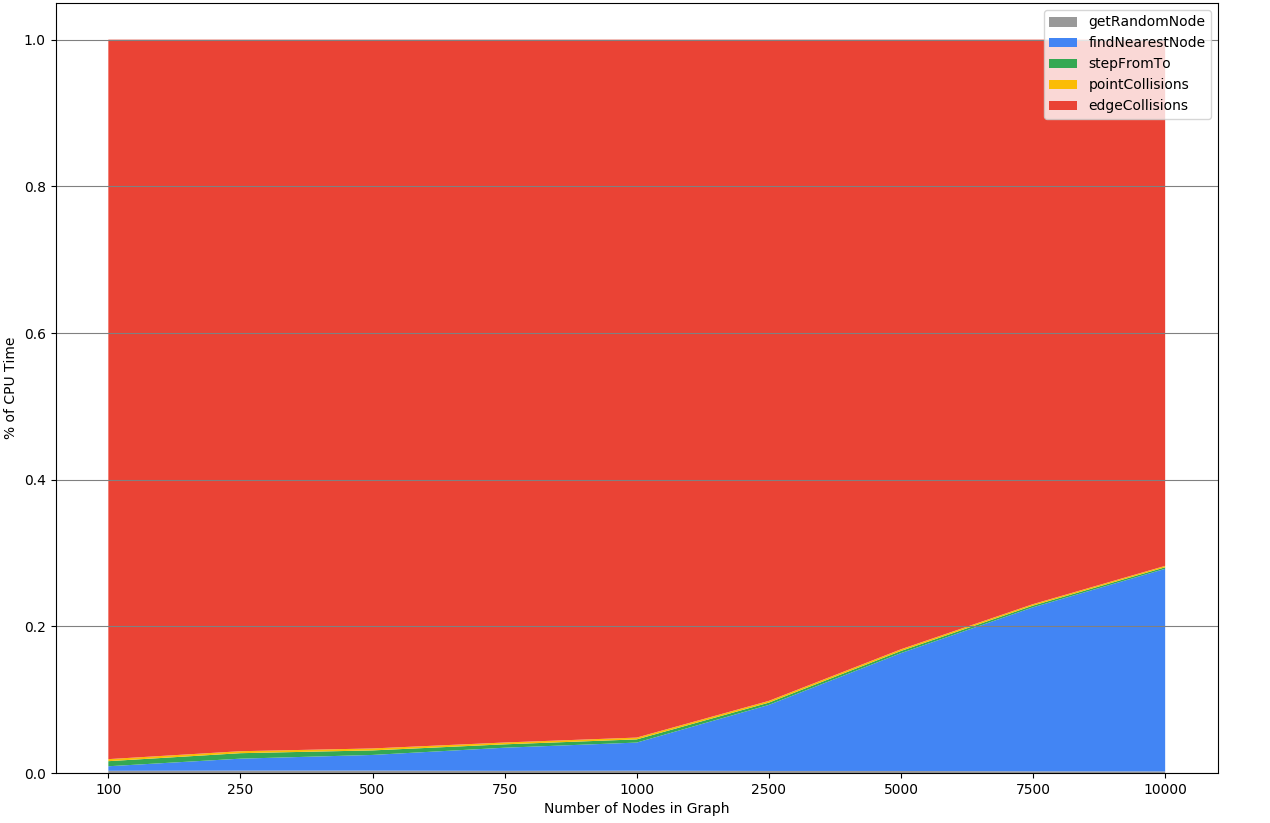
\includegraphics[width=\linewidth,height=0.3\paperheight]{chapters/chapter2/img/profiling/32x32x32/performance.png}
    \caption{32x32x32 Configuration Space}
    \label{subfig:32x32x32rrt}
    \end{center}
    \end{subfigure} 
    
    % Caption and Label
    \caption{\ac{RRT} Functions as a \% of Total CPU Exectution Time (cont.)}
    \label{fig:rrt_profiling}
\end{center}
\end{figure}
\todo[inline]{Change Y axis to \% and increase text size}

    Furthermore, the computational load of findNearestNode can be reduced through a variety of software optimizations. A simple one used here to demonstrate that fact is storing nodes in seperate ``buckets,'' sorted by their $x$ value. By using only two buckets, the execution time of findNearestNode fell drastically. Figure \ref{subfig:32x32x32rrt2} shows edge collision detection accounting for over 95\% of execution time for $100 \leq K \leq 10000$. This is consistent with the profiling results of \ac{RRT} in prior work\cite{Bialkowski2011}.

    \subsubsection*{Conclusion}
        From the above data, it was identified that, as prior work suggested, edge collision detection shows the greatest promise for potential speedup through specialized hardware. The next chapter details the process of designing and building this hardware.
        \todo[inline]{Add simulations to determine correct K}

    % @Author: AnthonyKenny98
% @Date:   2020-02-29 17:30:44
% @Last Modified by:   AnthonyKenny98
% @Last Modified time: 2020-03-01 08:08:09
\begin{figure}[H]
\begin{center}

    % Subfigure A
    \begin{subfigure}{\textwidth}
    \begin{center}
    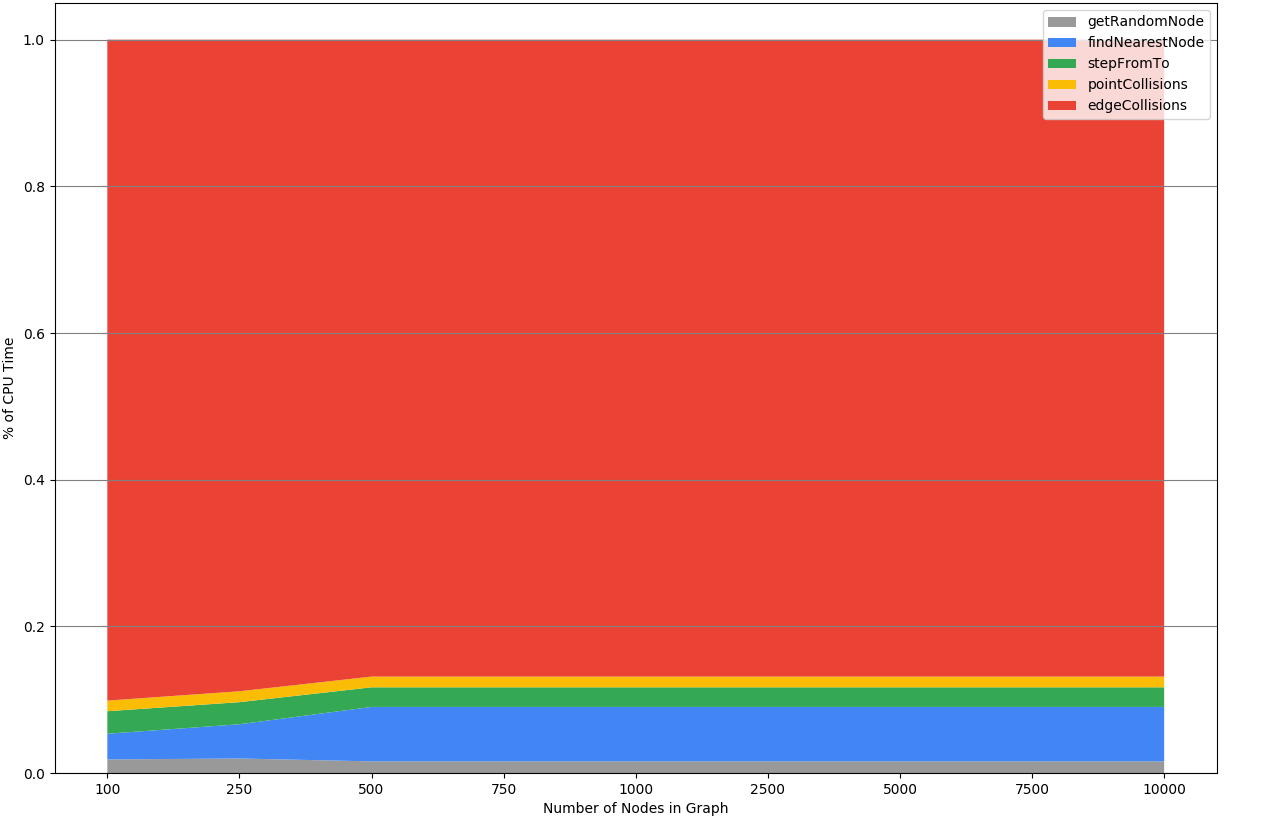
\includegraphics[width=\linewidth,height=0.3\paperheight]{chapters/chapter2/img/profiling/16x16x16/performance2.png}
    \caption{16x16x16 Configuration Space}
    \label{subfig:16x16x16rrt2}
    \end{center}
    \end{subfigure}
    % 
    % Subfigure B
    \begin{subfigure}{\textwidth}
    \begin{center}
    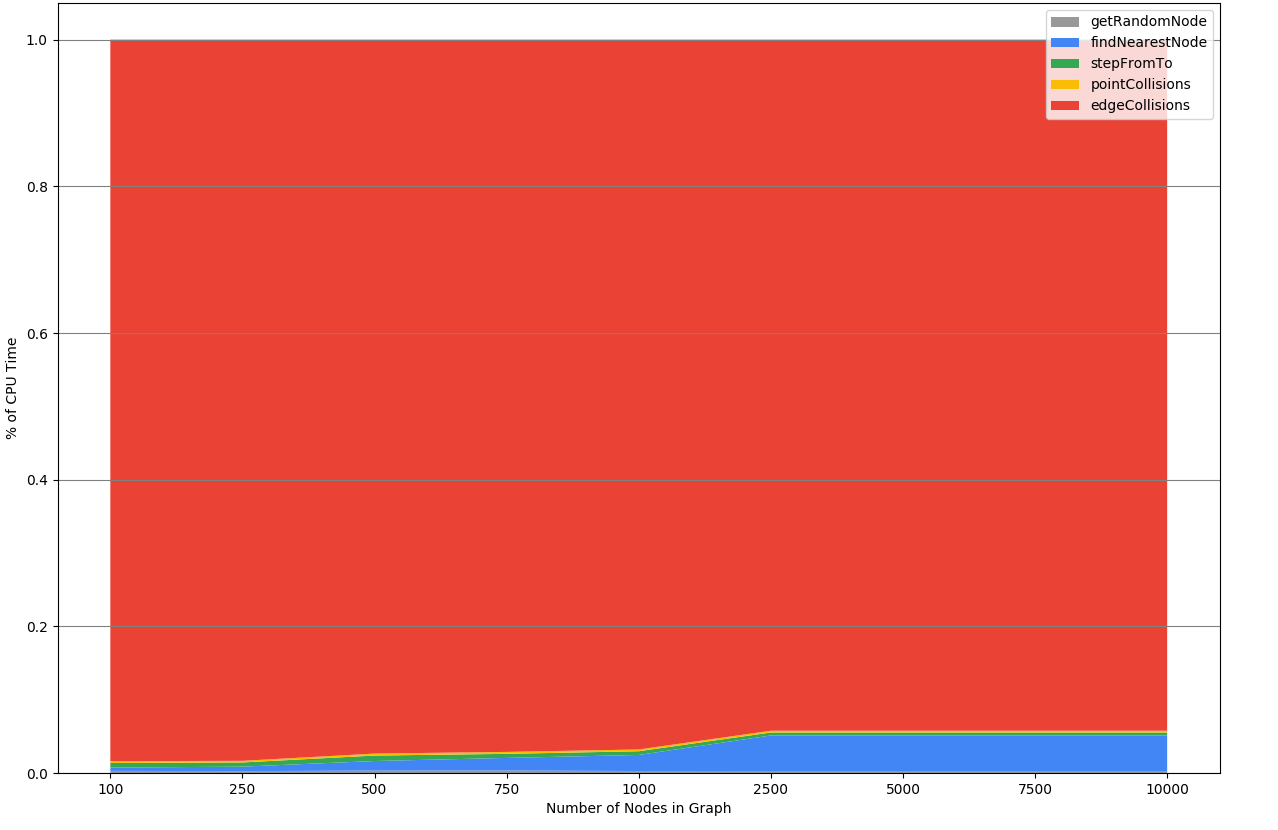
\includegraphics[width=\linewidth,height=0.3\paperheight]{chapters/chapter2/img/profiling/32x32x32/performance2.png}
    \caption{32x32x32 Configuration Space}
    \label{subfig:32x32x32rrt2}
    \end{center}
    \end{subfigure}
    % Caption and Label
    \caption{\ac{RRT} Functions Exectution Time, with Bucket Optimization}
    \label{fig:rrt_profiling2}
\end{center}
\end{figure}
